%%%%%%%%%%%%%%%%%%%%%%%%%%%%%%%%%%%%%%%%%
% Wenneker Assignment
% LaTeX Template
% Version 2.0 (12/1/2019)
%
% This template originates from:
% http://www.LaTeXTemplates.com
%
% Authors:
% Vel (vel@LaTeXTemplates.com)
% Frits Wenneker
%
% License:
% CC BY-NC-SA 3.0 (http://creativecommons.org/licenses/by-nc-sa/3.0/)
% 
%%%%%%%%%%%%%%%%%%%%%%%%%%%%%%%%%%%%%%%%%

%----------------------------------------------------------------------------------------
% PACKAGES AND OTHER DOCUMENT CONFIGURATIONS
%----------------------------------------------------------------------------------------

\documentclass[11pt]{scrartcl} % Font size

%%%%%%%%%%%%%%%%%%%%%%%%%%%%%%%%%%%%%%%%%
% Wenneker Assignment
% Structure Specification File
% Version 2.0 (12/1/2019)
%
% This template originates from:
% http://www.LaTeXTemplates.com
%
% Authors:
% Vel (vel@LaTeXTemplates.com)
% Frits Wenneker
%
% License:
% CC BY-NC-SA 3.0 (http://creativecommons.org/licenses/by-nc-sa/3.0/)
% 
%%%%%%%%%%%%%%%%%%%%%%%%%%%%%%%%%%%%%%%%%

%----------------------------------------------------------------------------------------
%	PACKAGES AND OTHER DOCUMENT CONFIGURATIONS
%----------------------------------------------------------------------------------------

\usepackage{amsmath, amsfonts, amsthm} % Math packages

\usepackage{listings} % Code listings, with syntax highlighting

\usepackage[english]{babel} % English language hyphenation

\usepackage{graphicx} % Required for inserting images
\graphicspath{{Figures/}{./}} % Specifies where to look for included images (trailing slash required)

\usepackage{booktabs} % Required for better horizontal rules in tables

\numberwithin{equation}{section} % Number equations within sections (i.e. 1.1, 1.2, 2.1, 2.2 instead of 1, 2, 3, 4)
\numberwithin{figure}{section} % Number figures within sections (i.e. 1.1, 1.2, 2.1, 2.2 instead of 1, 2, 3, 4)
\numberwithin{table}{section} % Number tables within sections (i.e. 1.1, 1.2, 2.1, 2.2 instead of 1, 2, 3, 4)

\setlength\parindent{0pt} % Removes all indentation from paragraphs

\usepackage{enumitem} % Required for list customisation
\setlist{noitemsep} % No spacing between list items

%----------------------------------------------------------------------------------------
%	DOCUMENT MARGINS
%----------------------------------------------------------------------------------------

\usepackage{geometry} % Required for adjusting page dimensions and margins

\geometry{
	paper=a4paper, % Paper size, change to letterpaper for US letter size
	top=2.5cm, % Top margin
	bottom=3cm, % Bottom margin
	left=3cm, % Left margin
	right=3cm, % Right margin
	headheight=0.75cm, % Header height
	footskip=1.5cm, % Space from the bottom margin to the baseline of the footer
	headsep=0.75cm, % Space from the top margin to the baseline of the header
	%showframe, % Uncomment to show how the type block is set on the page
}

%----------------------------------------------------------------------------------------
%	FONTS
%----------------------------------------------------------------------------------------

\usepackage[utf8]{inputenc} % Required for inputting international characters
\usepackage[T1]{fontenc} % Use 8-bit encoding

\usepackage{fourier} % Use the Adobe Utopia font for the document

%----------------------------------------------------------------------------------------
%	SECTION TITLES
%----------------------------------------------------------------------------------------

\usepackage{sectsty} % Allows customising section commands

\sectionfont{\vspace{6pt}\centering\normalfont\scshape} % \section{} styling
\subsectionfont{\normalfont\bfseries} % \subsection{} styling
\subsubsectionfont{\normalfont\itshape} % \subsubsection{} styling
\paragraphfont{\normalfont\scshape} % \paragraph{} styling

%----------------------------------------------------------------------------------------
%	HEADERS AND FOOTERS
%----------------------------------------------------------------------------------------

\usepackage{scrlayer-scrpage} % Required for customising headers and footers

\ohead*{} % Right header
\ihead*{} % Left header
\chead*{} % Centre header

\ofoot*{} % Right footer
\ifoot*{} % Left footer
\cfoot*{\pagemark} % Centre footer
 % Include the file specifying the document structure and custom commands
\usepackage{hyperref} % Include the hyperref package for URLs
\usepackage[backend=bibtex,style=numeric]{biblatex}
\usepackage{csquotes}
\usepackage{algorithm}
\usepackage{algpseudocode}
\addbibresource{Bibliography.bib} % Specify the bibliography file (ensure this file exists and contains entries)


%----------------------------------------------------------------------------------------
% TITLE SECTION
%----------------------------------------------------------------------------------------

\title{	
	\normalfont\normalsize
	\textsc{University of Galway}\\ % Your university, school and/or department name(s)
	\vspace{25pt} % Whitespace
	\rule{\linewidth}{0.5pt}\\ % Thin top horizontal rule
	\vspace{20pt} % Whitespace
	{\huge  Project 1: Evolutionary Search (GAs)}\\ % The assignment title
	\vspace{12pt} % Whitespace
	\rule{\linewidth}{2pt}\\ % Thick bottom horizontal rule
	\vspace{12pt} % Whitespace
}

\author{\LARGE Cathal Lawlor} % Your name

\date{\normalsize\today} % Today's date (\today) or a custom date

\begin{document}

\maketitle % Print the title

\section{Github Repository}
Github repository with code available \href{https://github.com/Laan33/ai_project_2}{here}

\section{Implementation details \& design choices}

\subsection{Tournament Selection and Mutation}
I used tournament selection for selecting parents for crossover. 
For my testing, I used a value of 5 for k, as it was a good balance between exploration and exploitation.
I used a mutation rate of 0.1, to allow for a good amount of exploration, but usually it did not result in significant deviations.

As I elaborate on later \ref{Training on all fixed strategies}, I had to implement an evaluation function where the score was the average of the agent competing against all the fixed strategies, as tournament selection would always discount any algorithms who were competed on the \texttt{Always Defect} strategy.

\subsection{Intialisation and Crossover}
I used a random initialisation for the population, with each gene being a random float between 0 and 1, representing the probability of cooperating given a certain history permutation.
I had a uniform crossover method, which randomly allocated a gene from either parent to the child.

\subsection{Termination condition}
I implemented a max number of generations to run, but I also added a clause, that if the algorithm hasn't improved by more than 0.015\% in the last 60 generations, it will terminate early.

This was to avoid the genetic algorithms getting stuck in local optima, or to stop when it had plateaued and there wasn't any changes.

\section{Part 1: Fixed strategies}
The agent had a memroy of 2, and only awareness of the enemys moves.

\subsection{Fixed strategies}
I trained the agent on the following fixed strategies:
\begin{itemize}
	\item \textbf{Always Cooperate} - Would always cooperate no matter what the agent did.
	\item \textbf{Always Defect} - Would always defect no matter what the agent did.
	\item \textbf{Tit for Tat} - Would do what the agent did on the previous turn.
	\item \textbf{Adaptive} - Always cooperate, unless the agent defected more than twice in the last 5 moves. 
	\item \textbf{Spiteful} - 30\% chance of defection the first turn, and had a (0.05 x num\_agent\_defections) probability of defection for all other moves (ignoring the agents first move).
\end{itemize}


\subsubsection{Generalised training on all fixed strategies}
\label{Training on all fixed strategies}
I trained a generalised agent on all the fixed strategies, with a generalised evaluation function.
I did this as tournament selection would always discount any algorithms who were trained on the \texttt{Always Defect} strategy.
Tournament selection wouldn't picked those agents, even if it was a perfect response to \texttt{Always Defect}, as it results in a really low payout relative to payouts other agents have when faced with 'easier' strategies. 

\begin{figure}[H]
	\centering
	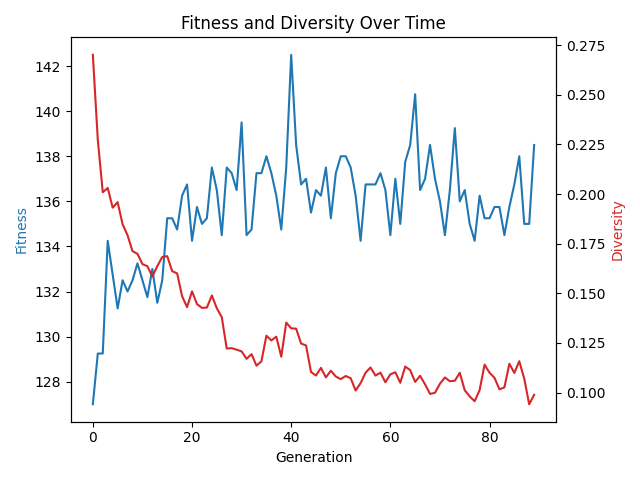
\includegraphics[width=0.8\linewidth]{Figures/part_1/generalised.png}
	\caption{Generalised Trained Alogrithm Tested On All Fixed Strategies}
	\label{fig:general_graph}
\end{figure}

\begin{table}[h!]
    \centering
    \begin{tabular}{|c|c|c|}
        \hline
		\textbf{(Fixed Strategy)} & \textbf{Agent Score} & \textbf{Fixed Strat Score} \\ \hline
        \textbf{Always Cooperate} & 172 & 117\\ \hline
        \textbf{Always Defect} & 50 & 50 \\ \hline
        \textbf{Tit-for-Tat} & 139 & 139 \\ \hline
        \textbf{Adaptive Strategy} & 167 & 122 \\ \hline
        \textbf{Spiteful Strategy} & 120 & 130 \\ \hline
    \end{tabular}
    \caption{Generalised agent performance against each fixed strategy}
    \label{tab:gen_agent_vs_fixed_strats}
\end{table}

With the stopping condition in place, the evolution stopped early at generation 89, as the fitness had plateaued, and the diversity of the population had converged.

As we can see, both in the graph\ref{fig:general_graph} and the results table\ref{tab:gen_agent_vs_fixed_strats}, 
the agent performed well against all the fixed strategies, except for the always cooperate strategy.

It isn't a surprise it struggled with the always cooperate strategy, as the agents training on the adaptive, spiteful and tit-for-tat strategies will have biased it's strategy for when an opponent has played \texttt{CC}. 
We can see this in the table\ref{tab:history_probabilities} representing the probability of the agent complying based on the opponent history.
If the memory was increased, it would almost certainly be able to differentiate the always cooperate strategy from the others.

The agent had a average fitness of 135.71, when averaged over all the fixed strategies 
(which however, isn't normalised for the different max possible results for each strategy), the table above, is a much better representation of the agent's performance.

% The best agent genome representation\ref{tab:history_probabilities} is:
\begin{table}[h!]
	\centering
	\begin{tabular}{|c|c|}
		\hline
		\textbf{(History permutation)} & \textbf{Probability of Cooperate} \\ \hline
		"" & 0.49 \\ \hline
		C & 0.86 \\ \hline
		D & 0.11 \\ \hline
		CC & 0.74 \\ \hline
		CD & 0.94 \\ \hline
		DC & 1.0 \\ \hline
		DD & 0.0 \\ \hline
	\end{tabular}
	\caption{Best generalised agent strategy genome}
	\label{tab:history_probabilities}
\end{table}

\subsubsection{Specific agents against other fixed strategies}

For fun, for each fixed strategy, I trained an agent against only that specific strategy, and then had the best evolved agent play all of the other strategies.

Some notable results: unsurprisingly, the \texttt{Always Cooperate} strategy performed well when it was tested against itself and the and \texttt{Always Defect} strategy, as it always was going to select the highest reward option, being always defect.
With this, it held it's own though against the other strategies.

The \texttt{Always Defect} strategy performed the worst, as it only knew what to do when the other agent defected twice in a row. 
The only wins it had were when the other potential combinations were used (e.g. DC, CC) and it happened to have a random value initialised that proved to be lucky.


The adaptive and tit for tat strategies are interesting to look at in how they performed.
\texttt{Tit-for-Tat} was quite compliant, and matched equal scores, except for when it was confused by \texttt{Always Defect} (as it not had any training experience with repeated \texttt{DD}).
\texttt{Adaptive Strategy} did well with \texttt{Always Cooperate}, but lost miserably out to \texttt{Always Defect}. Otherwise, it matched well for the other two tests.


\newpage
\section{Part 2: Extension}

\textbf{Disclaimer:} 
I didn't read the assignment spec initially and actually made a much more complex genome for part 1, and actually didn't have too much to extend for part 2. (I had a memory of 2, and probabilities rather than binary decisions)
Here is what I have changed:
\begin{itemize}
	\item Increased memory from 2 to 6.
	\item Good Samaritan Award
	\item Coevolution
\end{itemize}

\subsubsection{Memory increase}

\begin{figure}[H]
	\centering
	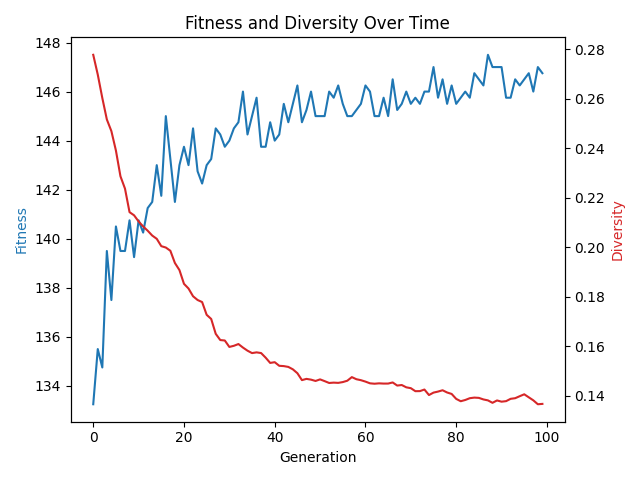
\includegraphics[width=0.8\linewidth]{Figures/part_2/extra_mem_gen.png}
	\caption{Generalised agent with more memory against Tested On All Fixed Strategies}
	\label{fig:extra_mem_gen_graph}
\end{figure}

I increased the memory from 2 to 6, as I wanted to see how the agent would perform with a larger memory.
It had a big impact on the agents performance, as it was able to differentiate between strategies much better, and was able to respond to the \texttt{Always Cooperate} strategy much better, as it wasn't being confused by other strategies like the \texttt{Spiteful} or \texttt{Adaptive} strategies.
It was able to differentiate between the \texttt{Always Cooperate} strategy and the

\begin{table}[H]
    \centering
    \begin{tabular}{|c|c|c|}
        \hline
		\textbf{(Fixed Strategy)} & \textbf{Agent Score} & \textbf{Fixed Strat Score} \\ \hline
        \textbf{Always Cooperate} & 248 & 3\\ \hline
        \textbf{Always Defect} & 49 & 54 \\ \hline
        \textbf{Tit-for-Tat} & 130 & 130 \\ \hline
        \textbf{Adaptive Strategy} & 140 & 110 \\ \hline
        \textbf{Spiteful Strategy} & 124 & 124 \\ \hline
    \end{tabular}
    \caption{Generalised agent with more memory, 100 generations}
    \label{tab:gen_mem_agent_vs_fixed_strats}
\end{table}

\newpage
\paragraph{Some notable pieces from the genome}
We can see how the algorithm was able to differentiate what to play for the \texttt{Always Cooperate} strategy, 
with a representation of \texttt{History: CCCCCC, Strategy Value: 0.0}, where it was always going to defect. This had it score 248, versus the 172 with the shorter memory.

For example then, with the \texttt{Spiteful Strategy} having a higher chance of initially defecting with a 0.3 probability (spiteful doesn't take into account the first agent move), the agent has learnt that if it keeps it's nose clean, the spiteful algorithm will keep cooperating.
At 5 moves, it has \texttt{History: DCCCC, Strategy Value: 0.91}, basically developing a strategy to try to keep working with spiteful, rather than have spiteful increase it's chance of defection (which spiteful will do for each agent defection).

\vspace{12pt} % Add vertical space
The first run \ref{tab:gen_mem_agent_vs_fixed_strats}, only had 100 generations to evolve with. 
Interestingly, when I removed the early stopping condition and had the agent evolve for 300 generations, 
it did not make any significant improvement, and performed worse in some instances - for example, against the spiteful algorithm.
\begin{table}[H]
    \centering
    \begin{tabular}{|c|c|c|}
        \hline
		\textbf{(Fixed Strategy)} & \textbf{Agent Score} & \textbf{Fixed Strat Score} \\ \hline
        \textbf{Always Cooperate} & 244 & 9\\ \hline
        \textbf{Always Defect} & 50 & 50 \\ \hline
        \textbf{Tit-for-Tat} & 138 & 133 \\ \hline
        \textbf{Adaptive Strategy} & 157 & 102 \\ \hline
        \textbf{Spiteful Strategy} & 91 & 126 \\ \hline
    \end{tabular}
    \caption{Generalised agent, more memory, 300 generations of evolution.}
    \label{tab:300_gen_mem_agent_vs_fixed_strats}
\end{table}

\subsection{Good Samaritan Award}
I added an award to the agent, that will reward it with the \texttt{num\_round x 3.5} of the score, if it only has only cooperated on every turn.
This would also happen in only 55\% of the cases.

This means, it will have it will have the slightly better than the max possible reward.
I did this, as I was interested in what would the agent do, and how the diversity would hold up.


\begin{figure}[H]
    \centering
    \begin{minipage}{0.45\textwidth}
        \centering
        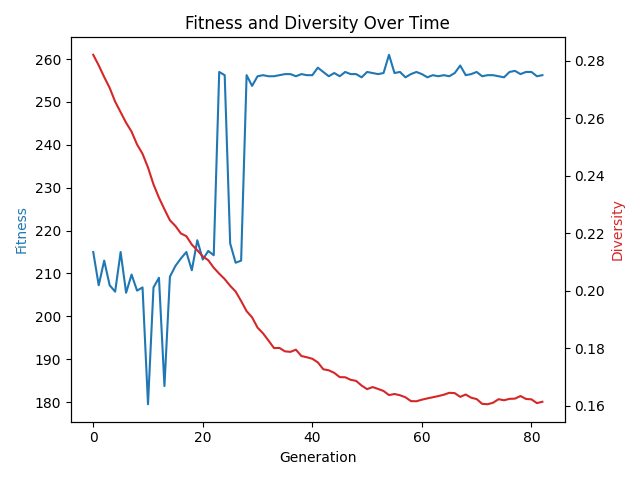
\includegraphics[width=\linewidth]{Figures/part_2/good_samaritan/plot_2025-03-11 19-31-27_0.png}
    \end{minipage}\hfill
    \begin{minipage}{0.45\textwidth}
        \centering
        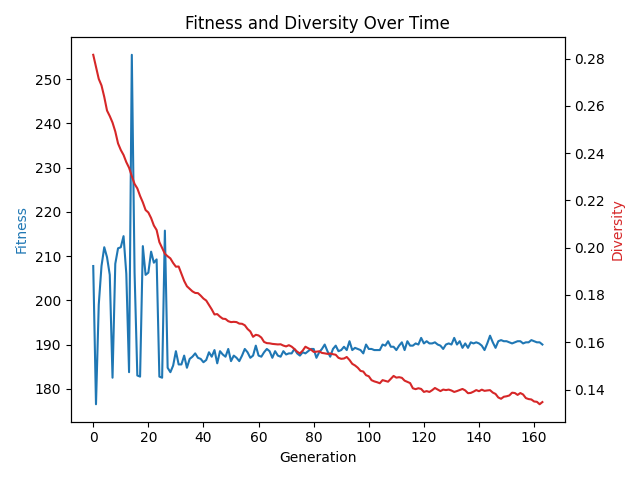
\includegraphics[width=\linewidth]{Figures/part_2/good_samaritan/plot_2025-03-11 19-31-27_1.png}
    \end{minipage}
    \begin{minipage}{0.45\textwidth}
        \centering
        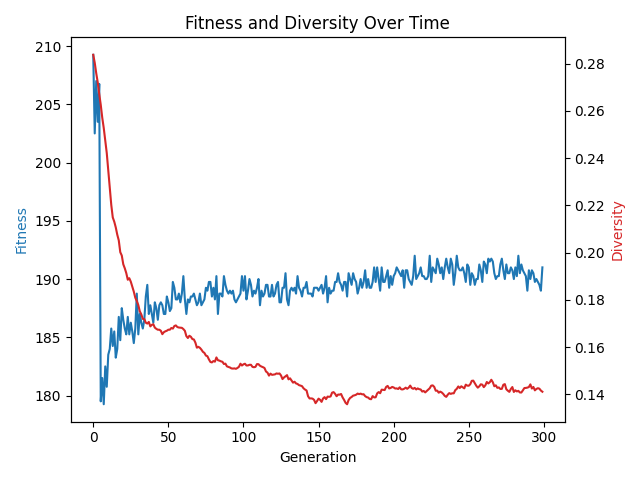
\includegraphics[width=\linewidth]{Figures/part_2/good_samaritan/plot_2025-03-11 19-31-27_2.png}
    \end{minipage}\hfill
    \begin{minipage}{0.45\textwidth}
        \centering
        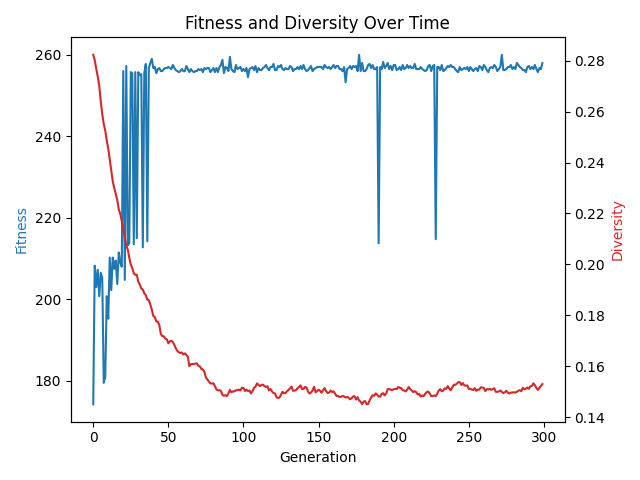
\includegraphics[width=\linewidth]{Figures/part_2/good_samaritan/plot_2025-03-11 19-31-27_3.png}
    \end{minipage}
	\caption{Good Samaritan Award Testing}
	\label{fig:good_samaritan_award}
\end{figure}

With the good samaritan configuration, I evolved the agent for 300 generations, with a memory of 6.
As you can see in the above figure \ref{fig:good_samaritan_award}, from 4 runs, twice did the agent evolve to find the higher reward system, and twice did it actually find it, but then evolve to not take advantage of it.

Additionally you can also see where the agent found the higher reward system, accidentally evolved to not take advantage of it, but quickly re-evolved to take advantage of it again.

The diversity score of the populations isn't noticably any different to other runs without this 'good samaritan' award, where as per usual, the diversity converges at around generation 40.
From this, the reward system is a highly divise factor in the population, and the agent will either quickly adapt to it or shun it.


\section{Coevolution}
With the two other enhancements, I wanted to see how the agent would perform in a coevolutionary setting.

I firstly ran the coevolutionary training with just the increased memory, where it initially plunges in performance, but slowly recovers back to a reasonable score.
As the agent irons out the random noise in it's initial population, it starts to perform better where it will sometimes give itself a higher reward (by accident probably), which is worth more than just continually defecting.

\begin{figure}[H]
	\centering
	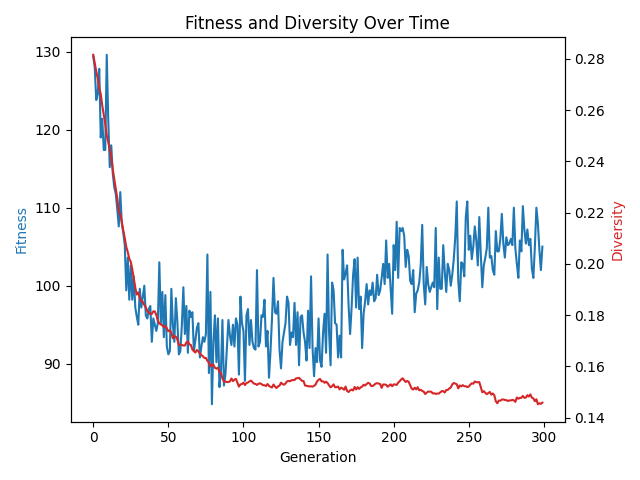
\includegraphics[width=0.8\linewidth]{Figures/part_2/no_good_sam_coev/300.png}
	\caption{Coevolutionary training with increased memory}
	\label{fig:300_gen_mem_coev}
\end{figure}

I then ran the coevolutionary training with the good samaritan award, and the increased memory.
The agents did not engage with the good samaritan award with it's initial implementation at all.

I removed the probability element, awarding it everytime that the agent had a run with no more than 3 defections. This still had little impact, so I decreased the round count from 50 to 15.

Only then did the agents start to engage with the good samaritan award.
\begin{figure}[H]
    \centering
    \begin{minipage}{0.45\textwidth}
        \centering
        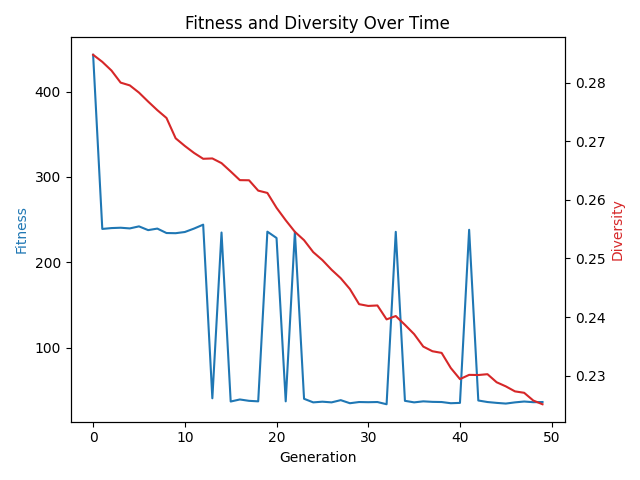
\includegraphics[width=\linewidth]{Figures/part_2/goodSamC1.png}
    \end{minipage}\hfill
    \begin{minipage}{0.45\textwidth}
        \centering
        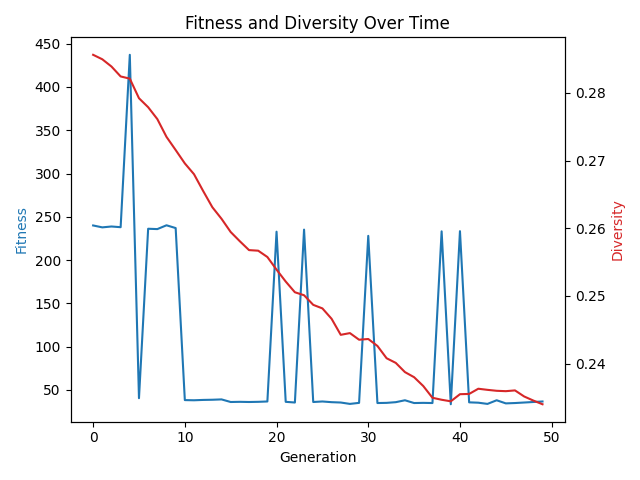
\includegraphics[width=\linewidth]{Figures/part_2/goodSamC22.png}
    \end{minipage}
	\begin{minipage}{0.45\textwidth}
        \centering
        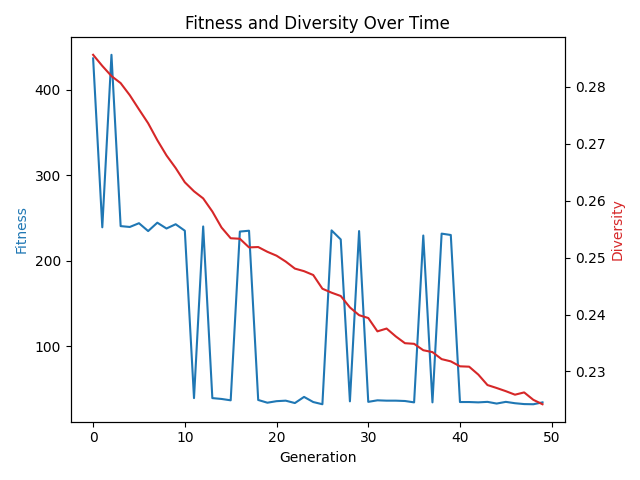
\includegraphics[width=\linewidth]{Figures/part_2/goodSamC3.png}
    \end{minipage}
	\label{fig:coev_good_samaritan_award}
	\caption{Coevolutionary training with good samaritan award}
\end{figure}

Even after all the changes, the agents still usually didn't engage with the good samaritan award on every run, and would evolve away from an initial position of achieving it for around 10 generations.

I guess from this, my agents are just too selfish to be good samaritans ;)

\subsection{Coevolution against each other}
%  Total scores: {<__main__.IPDGenotype object at 0x118480250>: 318, <__main__.IPDGenotype object at 0x1187a54f0>: 298, <__main__.IPDGenotype object at 0x11889db50>: 321, <__main__.IPDGenotype object at 0x1189a2700>: 321, <__main__.IPDGenotype object at 0x118a82310>: 314}
Running without all the good samaritan changes, I pitted 5 coevolutionary agents against each other.
Surprisingly, I found that the agents did not just always defect against one anohter, and had quite close scores.
The agents were able to find a balance between defecting and cooperating, resulting in higher payoffs overall and not just getting the worst score from both defecting.
The scores in order of the agents were: 321, 321, 318, 314, 298.

\section{Conclusion}


I had good fun with this mini project.

Coevolutionary training was interesting, as it was able to find a balance between themselves to result in higher payoffs, even if it meant losing out to itself for the odd turn.

The effects of the memory size difference also were insightful, as it opened up a lot more nuanced strategies.
If I had more time, I would have liked to have seen how the agents would have performed with an awareness of it's own moves, and not just the opponents.
(although, you will have to make sure the memory doesn't become too large, as it will scale really badly with the number of possible history permutations). This does lead into an idea space that basically is one of using a neural network to approximate the strategy, (which would be interesting in it's own right).

% \section{Potential improvements}
% \label{Potential improvements}


% One easy, improvment I believe for my algorithm would be to employ elitism.
% I implemented it in a early version of the program. I chose not to implement it, as I wanted to see how the various methods for crossover and mutation would handle the problem alone, without the help of elitism.
% It would probably extract a small bit more performance out, especially for the bigger datasets, less so in the Berlin dataset.

% I believe that tournament selection is a good choice, being the sweet spot for a genetic algorithm solving TSP. It's fast, simple, and maintains a good diversity and doesn't suffer with early convergence like roulette wheel selection can\cite{genetic_algorithm_afternoon}.
% I also tried monte carlo selection, but I do not believe it works for the travelling salesperson problem.

% Another, is to run the same parameters multiple times on differening starting populations, and averaging the results. This would give a more accurate representation of the algorithm's performance, as the starting population can have a big impact on the final result. e.g. it may get stuck in a local optima, or converge too early.
% Also related to this, is to allow the algorithm to do hyperparameter tuning on the fly (e.g. using adaptive mutation or crossover rates based on fitness), as it's running. This would allow the algorithm to adjust to the problem, and the population, as it's running, and not just at the start.

% For the bigger pr1002 dataset, I think given more time and resources would help improve the results on the large pr1002 dataset. 
% Mainly, this would allow me to up the population size by a lot, which then allows it to run for a lot more generations without converging too early, allowing more exploraiton of the solution space.

% There is other improvements, such as a hybrid approach of a local search algorithm, e.g. 2-opt, to improve the final solution once the genetic algorithm has converged. This would help fine-tune the solution, and get a better result.

\printbibliography
\end{document}
